% Question 1 fragment. Needs: \usepackage{amsmath,amssymb,booktabs,longtable,array,graphicx}
% Figure: run `python q1_diagram.py` -> figures/q1_architecture.png
\section*{Question 1 --- River Forecasting Proposal}

\noindent\textbf{Summary.} A small multimodal \emph{river-graph forecaster}. Each monitored node
(reservoir release, S1--S4, T1) is encoded by a shared recurrent network; information is exchanged
only along the directed river links through \emph{lag attention} (so the effective travel time adapts to
current conditions); the decoder adds the announced future releases and outputs the 10th/50th/90th
percentile water level at S1--S4 for the next six 10-minute steps. The model forecasts \emph{changes
relative to the latest observed level}, so physical persistence is built in and learning only has to
explain the evolution.

%==========================================================================
\subsection*{1. Architecture diagram}
\begin{center}
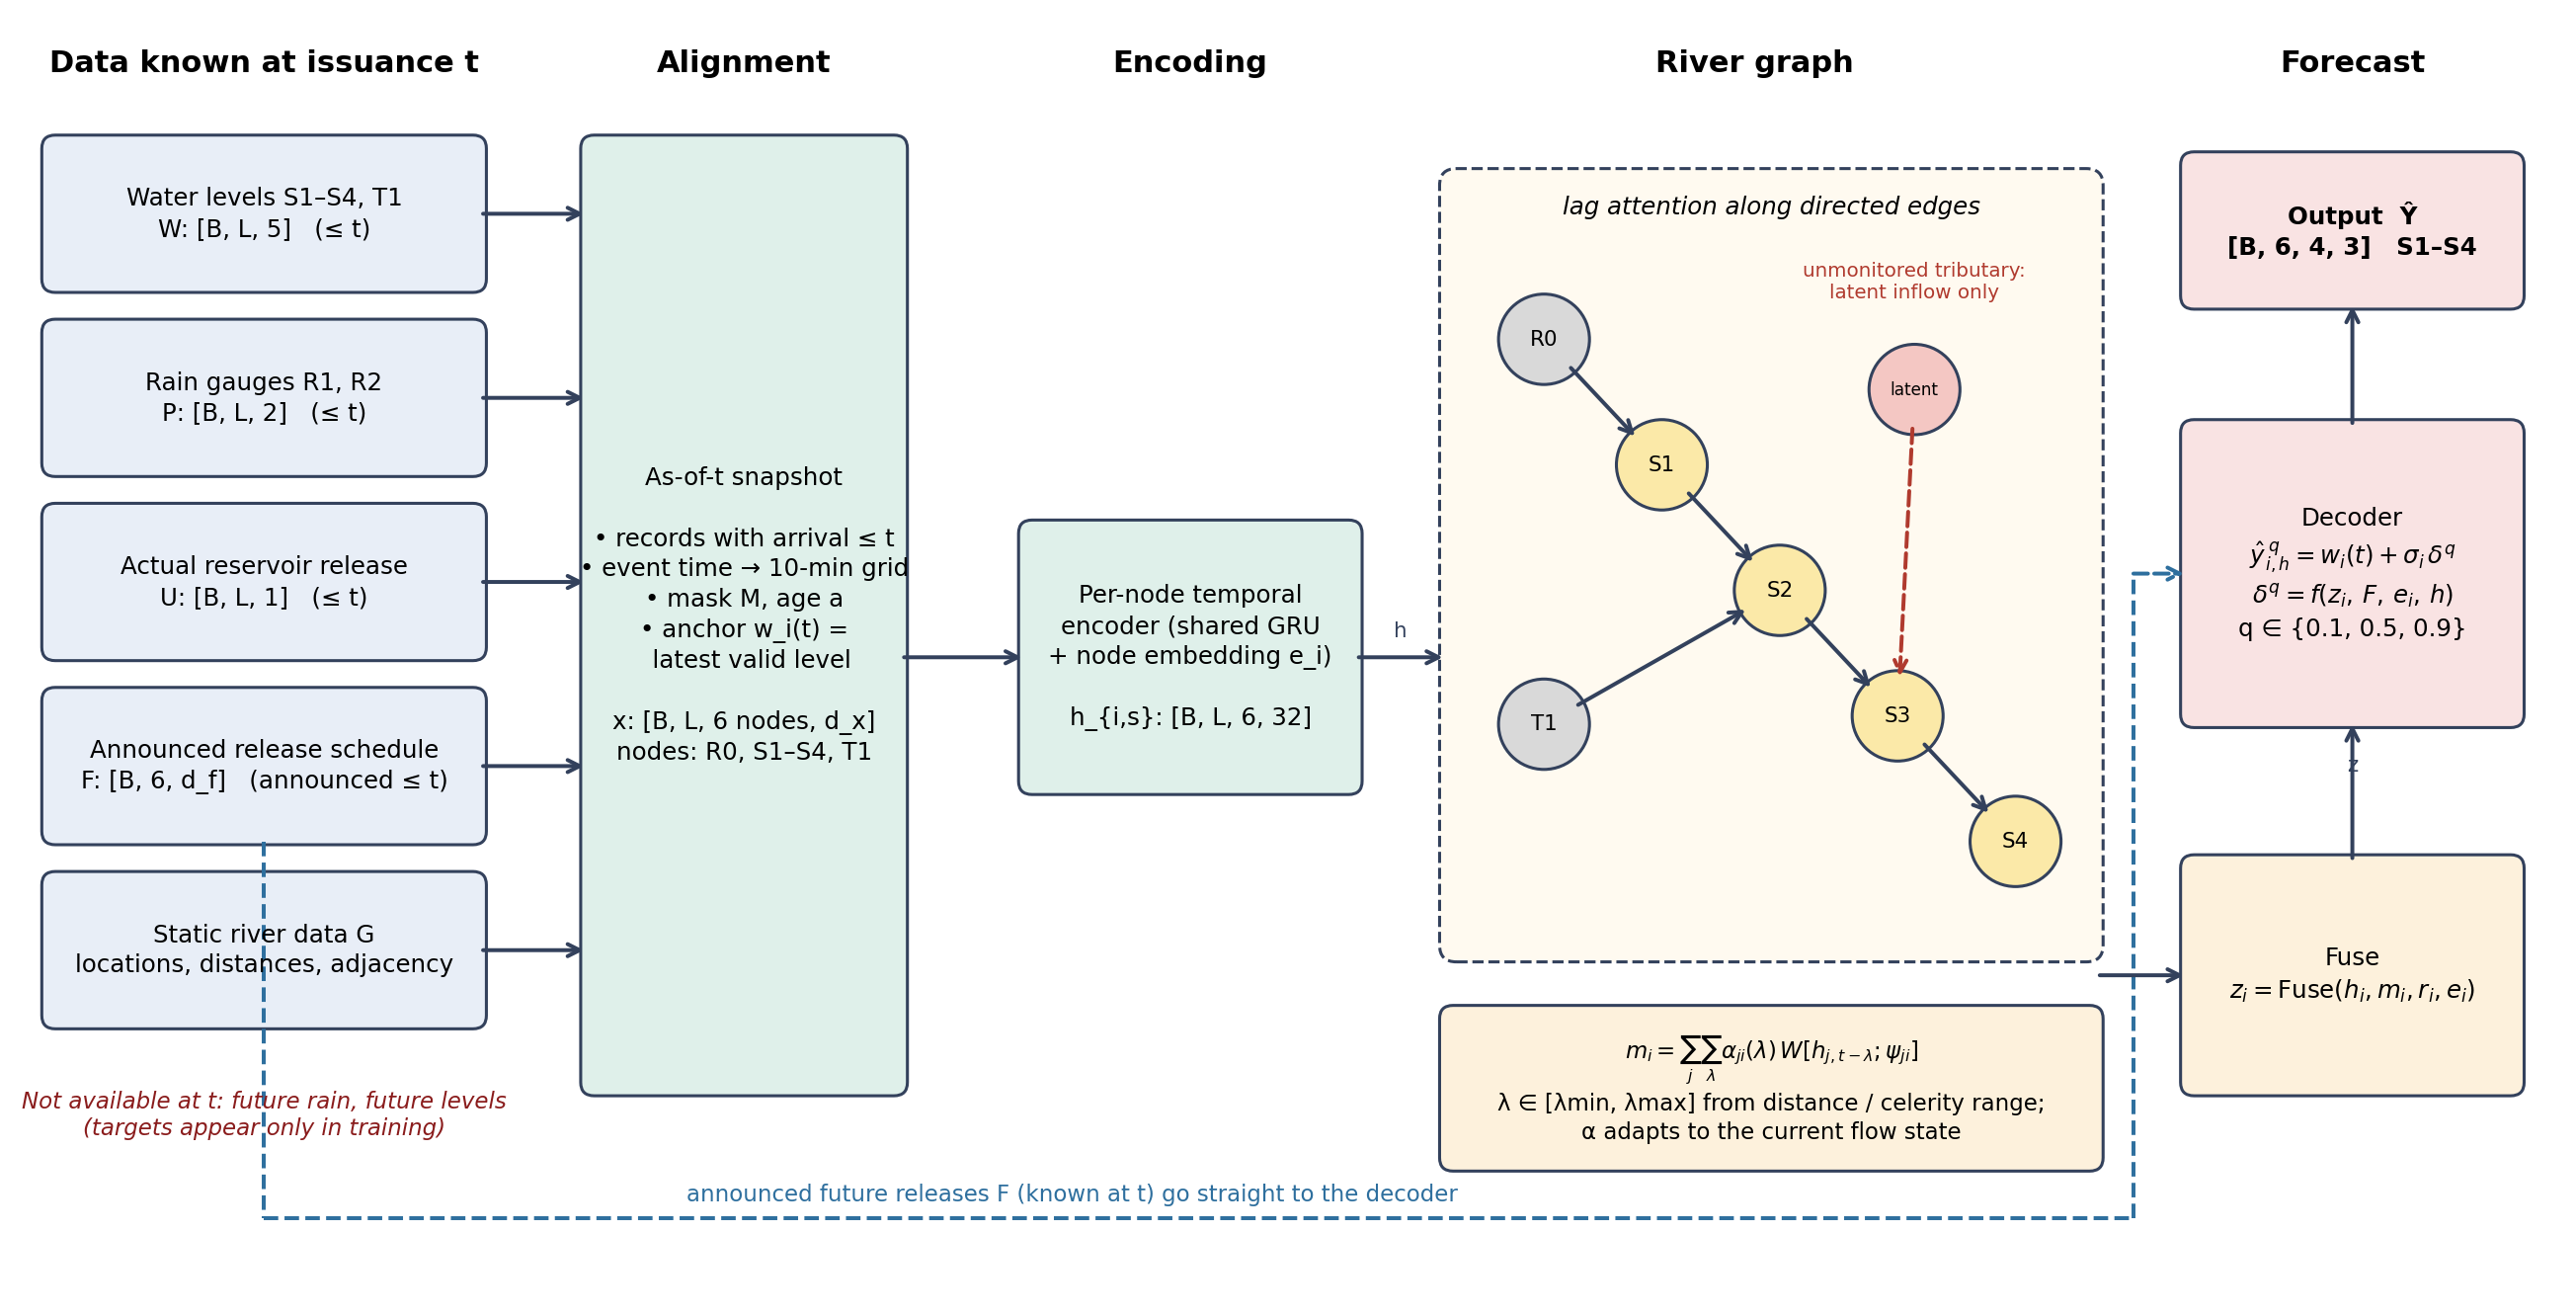
\includegraphics[width=\linewidth]{figures/q1_architecture.png}
\end{center}
\noindent\textit{Figure Q1.} Data sources (left) are aligned to an as-of-issuance snapshot with masks and
ages; a shared GRU encodes every node; lag attention moves information downstream along
R0$\to$S1$\to$S2$\to$S3$\to$S4 and T1$\to$S2; the unmonitored tributary enters only as a latent residual
at S3; announced future releases enter the decoder; the output is $\hat Y\in\mathbb R^{B\times 6\times 4\times 3}$
(batch $\times$ horizon $\times$ station $\times$ quantile). Future rainfall and future levels are never inputs.

%==========================================================================
\subsection*{2. Assumptions}
\noindent\textbf{Supplied facts (not assumptions).}
\textbf{F1} Forecast every 10 minutes, one hour ahead, at S1--S4.
\textbf{F2} Available data: history of S1--S4 and T1 levels (10-min); R1, R2 rainfall with timestamps and
locations; recorded reservoir releases and announced future release schedules (with announcement and effective
times); station locations, river connectivity and along-river distances.
\textbf{F3} A monitored tributary joins between S1 and S2 (gauged at T1); an unmonitored one joins between S2 and S3.
\textbf{F4} Travel times and unmonitored inflow are not supplied; stations are unevenly spaced; travel times vary
with river conditions. \textbf{F5} Future rainfall and future levels are unavailable at issuance; extra information
may be requested but is not guaranteed.

\medskip
\noindent\textbf{Assumed details} (each states what is assumed, why it is reasonable, and its effect on the design).
\small
\begin{longtable}{@{}p{0.05\linewidth}p{0.30\linewidth}p{0.30\linewidth}p{0.30\linewidth}@{}}
\toprule
 & \textbf{Assumption} & \textbf{Why reasonable} & \textbf{Effect on design}\\ \midrule\endhead
A1 & All level series lie on a common 10-min grid; timestamps within $\pm5$ min are snapped to the nearest slot. & F2 states a 10-min cadence; real loggers drift by seconds--minutes. & One time axis for all nodes; no interpolation between stations.\\
A2 & $\geq 2$ years of history including at least one flood season, $<5\%$ of values missing. & Needed for any learned model; record length is not specified. & Chronological train/validation/test split; performance on rare extremes is reported as uncertain (Sec.~6).\\
A3 & Records usually arrive within 0--2 slots; outages of hours occur; arrival timestamps $\nu_r$ are logged (otherwise simulated). & Typical telemetry behaviour; unspecified in the brief. & Inputs carry mask and age; training uses the as-of snapshot.\\
A4 & Sensor noise is small relative to 1-h level changes; spikes are flagged by quality control. & Hydrograph changes over an hour are usually larger than gauge noise. & Robust (pinball) loss; flagged values are treated as missing.\\
A5 & Flow influence is downstream; backwater from the town/bridge below S4 does not affect S1--S4 within the horizon. & Rivers are advection-dominated at this scale. & Edges are directed; no S4$\to$S3 edge.\\
A6 & Travel time varies with flow but stays within $[\lambda_{\min},\lambda_{\max}]$ per reach, derived from the along-river distance and a plausible wave-celerity range $c\in[c_{\min},c_{\max}]$, later tightened from lagged cross-correlation of the history. & F4: not constant, not supplied; a bounded window is the weakest useful prior. & Lag attention over a bounded window (Sec.~4) instead of one fixed delay.\\
A7 & Gauges R1, R2 are point proxies for catchment rain; runoff reaches a station after a delay of tens of minutes to hours; R2 (from the illustration, not to scale) is the nearer proxy to the unmonitored tributary. & Rain is only measured at two points. & Rain reaches each node through learned gauge weights $\beta_{ig}$ based on location features.\\
A8 & An announced schedule is intent, not a guarantee; revisions arrive as new announcements. & F2 gives announcement \emph{and} effective times, implying revisions. & Schedule snapshot as of $t$; deviation from actual release is a feature (Sec.~5).\\
A9 & The reservoir release is the main controllable boundary condition of S1; other lateral gains/losses are small. & Only listed influences are given. & Release enters through a dedicated node R0.\\
A10 & The unmonitored inflow is driven mostly by rain in its own catchment and is smooth within one hour except in storms. & Standard rainfall--runoff behaviour. & Modelled as a latent residual at S3 with wider intervals (Sec.~4, 6).\\
A11 & The target is stage (level); level--discharge relations are monotone and stable over the deployment period. & Stage is what is measured and what warnings use. & No discharge conversion; periodic retraining handles slow changes.\\
A12 & Distribution is stationary enough that a model trained on past years is valid, re-trained periodically. & Needed for any data-driven system. & Monitoring and retraining are part of operation (Sec.~5).\\
\bottomrule
\end{longtable}
\normalsize

%==========================================================================
\subsection*{3. Forecasting task and data specification}
\noindent\textbf{Task.} Issuance times lie on the 10-minute grid, $t=n\Delta$, $\Delta=10$ min. History window:
$L=288$ slots (48 h), i.e.\ slots $t-L+1,\dots,t$. Horizon: $H=6$ steps, $t+h\Delta$, $h=1,\dots,6$.
Outputs: levels at S1--S4 for each horizon; point forecast = median.
Nodes: $\mathcal N=\{R0,S1,S2,S3,S4,T1\}$ (R0 = reservoir release; T1 is input-only). Batch axis $B$ = number of
issuance times in a mini-batch.

\small
\begin{center}
\begin{tabular}{@{}p{0.17\linewidth}p{0.17\linewidth}p{0.34\linewidth}p{0.24\linewidth}@{}}
\toprule
\textbf{Tensor} & \textbf{Shape} & \textbf{Axes} & \textbf{Time coverage}\\ \midrule
Levels $W$ + mask $M^W$ + age $a$ & $[B,L,5]$ each & batch; history slot; channel (S1,S2,S3,S4,T1) & $t-L+1\ldots t$, only records with arrival $\le t$\\
Rain $P$ + mask & $[B,L,2]$ & batch; slot; gauge (R1,R2); 10-min accumulation over $(\tau-\Delta,\tau]$ & $t-L+1\ldots t$\\
Actual release $U$, and its schedule at that time $U^{\rm sch}$ & $[B,L,1]$ each & batch; slot; scalar release (last value held between records) & $t-L+1\ldots t$\\
Future schedule $F$ & $[B,H,d_f]$ & batch; forecast step; (scheduled release, availability flag, lead since announcement) & effective times $t+\Delta\ldots t+6\Delta$; announced $\le t$\\
Static $G$ & $[4,d_s]$ + adjacency & node; location, order, along-river distances $d_{ji}$ & fixed\\
Encoded input $x$ & $[B,L,6,d_x]$ & batch; slot; node; features after alignment & as above\\
Output $\hat Y$ & $[B,6,4,3]$ & batch; horizon $h$; station; quantile $q\in\{0.1,0.5,0.9\}$ & $t+\Delta\ldots t+6\Delta$\\
Target $Y$ (training only) & $[B,6,4]$ & batch; horizon; station & never an input\\
\bottomrule
\end{tabular}
\end{center}
\normalsize

\noindent\textbf{Alignment.} \emph{Sampling times:} levels are on the grid (A1); rainfall readings, stamped with event time, are summed
into the 10-min bin containing them; releases are step functions sampled at each slot (last value held); schedules keep
$(a_k,e_k,e_k^{\rm end},r_k)$ = announcement, effective start/end, value. \emph{Locations:} values are attached to nodes, never interpolated between
stations; gauges are linked to nodes through the learned weights below. \emph{As-of snapshot:} for issuance $t$ only records with arrival
time $\nu\le t$ and schedules with $a_k\le t$ are used; this prevents future leakage in training and in operation.

\noindent\textbf{Known at issuance:} all history above, the announced schedule, static data. \textbf{Unknown:} future rain, future levels,
tributary inflow, unannounced release changes.

%==========================================================================
\subsection*{4. Model computations and design justification}
\noindent\textbf{Notation.} Node $i\in\mathcal N$, slot $s$; level $w_{i,s}$, mask $m_{i,s}\in\{0,1\}$, age $a_{i,s}$ (minutes since the last
valid value). Normalised level $\tilde w_{i,s}=(w_{i,s}-\mu_i)/\sigma_i$ (training statistics). Anchor $w_i(t)$ = latest valid level of station $i$.

\noindent\textbf{(a) Rain to node.} $r_{i,s}=\sum_{g\in\{R1,R2\}}\beta_{ig}\tilde P_{g,s}$, $\beta_{i\cdot}=\mathrm{softmax}_g\big(\mathrm{MLP}_\beta(\psi^{\rm rain}_{ig})\big)$,
with $\psi^{\rm rain}_{ig}$ the location features (distance along/across the river). Node inputs:
$x_{i,s}=[\tilde w_{i,s},\,m_{i,s},\,a_{i,s}/a_{\max},\,\tilde w_{i,s}-\tilde w_{i,s-1},\,r_{i,s}]$ for stations and T1;
$x_{R0,s}=[\tilde U_s,\,m,\,a,\,\tilde U_s-\tilde U^{\rm sch}_s]$.

\noindent\textbf{(b) Temporal encoder (shared weights).}
$h_{i,s}=\mathrm{GRU}_\theta\big(h_{i,s-1},[x_{i,s};e_i]\big)\in\mathbb R^{d}$, $d=32$, $h_{i,t-L}=0$; $e_i$ is a learned node embedding;
$h_i:=h_{i,t}$.

\noindent\textbf{(c) River message passing with lag attention.} Edges $\mathcal E=\{(R0,S1),(S1,S2),(T1,S2),(S2,S3),(S3,S4)\}$.
For edge $(j,i)$ with distance $d_{ji}$, the admissible lags (in slots) are
$\Lambda_{ji}=\{\lambda:\lceil d_{ji}/(c_{\max}\Delta)\rceil\le\lambda\le\lceil d_{ji}/(c_{\min}\Delta)\rceil\}$ (A6). With $\psi_{ji}$ = edge features and $\phi(\cdot)$ a sinusoidal lag code,
\begin{align}
k_{ji\lambda}&=W_k[h_{j,t-\lambda};\psi_{ji};\phi(\lambda)],\quad q_i=W_q h_i,\\
\alpha_{ji}(\lambda)&=\mathrm{softmax}_{\lambda\in\Lambda_{ji}}\!\big(q_i^{\!\top}k_{ji\lambda}/\sqrt{d_k}\big),\\
m_i&=\sum_{(j,i)\in\mathcal E}\ \sum_{\lambda\in\Lambda_{ji}}\alpha_{ji}(\lambda)\,W_v[h_{j,t-\lambda};\psi_{ji}].
\end{align}
The query depends on the downstream node's current state (e.g.\ current level and rate), so the attended lag shifts when the river is high or low:
a learned, flow-dependent travel time restricted to a physically bounded window.

\noindent\textbf{(d) Unmonitored tributary.} At S3 only, a latent residual $u_3=g_\theta\big([h_3-\mathrm{Proj}(m_3);\,r_3]\big)$ is added, $m_3\leftarrow m_3+u_3$:
the part of S3's recent behaviour that neither upstream S2 nor local rain explains. It is never supervised directly; it is identified only through the forecast loss, which is why it is paired with wider intervals (Sec.~6).

\noindent\textbf{(e) Fusion.} $z_i=\mathrm{LN}\big(h_i+\mathrm{MLP}_f([h_i;m_i;r_{i,t};e_i])\big)$, $i\in\{S1,\dots,S4\}$.

\noindent\textbf{(f) Forecast mapping with announced releases.} Let $\tilde u_s=\tilde U_s$ for $s\le t$ and $\tilde u_s=\tilde U^{\rm sch}_s$ for $s>t$, with flag $f_s=\mathbb 1[s>t]$.
For horizon $h$, reservoir water released at slot $s$ reaches station $i$ about $\lambda\in\Lambda_{R0,i}$ slots later, so
\begin{align}
\gamma_{i,h}(\lambda)&=\mathrm{softmax}_{\lambda}\,\mathrm{MLP}_a([z_i;\phi(h);\phi(\lambda)]),\quad
g_{i,h}=\sum_{\lambda}\gamma_{i,h}(\lambda)\,[\tilde u_{t+h-\lambda};\,f_{t+h-\lambda}],\\
\delta^{0.5}_{i,h}&=\mathrm{MLP}_{\rm dec}([z_i;g_{i,h};e_i;\phi(h)]),\quad
\delta^{0.1}_{i,h}=\delta^{0.5}_{i,h}-\mathrm{softplus}(\cdot),\quad \delta^{0.9}_{i,h}=\delta^{0.5}_{i,h}+\mathrm{softplus}(\cdot),\\
\hat y^{\,q}_{i,h}&=w_i(t)+\sigma_i\,\delta^{q}_{i,h}.
\end{align}
(Quantiles are monotone by construction; announced releases that take effect before reaching the station are exactly the ``known future'' information.)

\noindent\textbf{(g) Training objective.} With $\rho_q(e)=\max(qe,(q-1)e)$ and $\Omega$ the set of (issuance $t$, station $i$, horizon $h$) with an observed target,
\[
\mathcal L=\frac1{|\Omega|}\sum_{(t,i,h)\in\Omega}\ \frac1{\sigma_i}\sum_{q\in\{0.1,0.5,0.9\}}\rho_q\!\big(y_{i,h}(t)-\hat y^{\,q}_{i,h}(t)\big).
\]
Training windows use every 10-min issuance time of the training period (chronological split), the schedule \emph{as announced at that time},
and random mask/delay augmentation (Sec.~5). Coverage of $[q_{0.1},q_{0.9}]$ is checked on validation per station and horizon and recalibrated if needed.

\noindent\textbf{How each influence enters the forecast.}
\emph{Upstream conditions:} lagged encoder states of the upstream node through $\alpha_{ji}$ (and the anchor $w_i(t)$).
\emph{Tributary T1:} an extra upstream edge into S2, so T1's rise reaches S2 after its own lag window and carries on to S3 and S4 through S2's state.
\emph{Rainfall:} node-wise $r_{i,s}$ (local response) plus the latent term at S3 (unmonitored basin).
\emph{Reservoir releases:} past actual releases through the R0$\to$S1 edge; announced future releases through $g_{i,h}$ in the decoder.

\noindent\textbf{Physical versus learned.} \emph{Physical/structural (fixed):} directed downstream topology; causality (no S4$\to$S3 edge); lag windows bounded by distance/celerity (A6); anchoring to the last observed level;
no use of unavailable future data; quantile ordering. \emph{Learned:} actual lag weights within the window, rain-to-level response and gauge weights $\beta$,
release attenuation/delay, the unmonitored inflow residual, level-dependent behaviour, and the interval widths. No separate hydraulic simulator is used (optional per the brief).

\noindent\textbf{Why this design.} Directed message passing uses the supplied river structure instead of a flat network over all inputs (which would have to rediscover topology
and would transfer poorly between stations); a bounded learned lag window addresses changing travel times better than a fixed delay; predicting increments from the latest level
is a strong baseline over 1 h; quantile outputs express uncertainty without a separate probabilistic model; parameter count is small ($\sim10^{5}$), which suits limited history and 10-minute operation.

%==========================================================================
\subsection*{5. Operation and exceptional conditions}
\small
\begin{longtable}{@{}p{0.17\linewidth}p{0.80\linewidth}@{}}
\toprule\endhead
\textbf{(i) Missing observations} & If a node's value is absent at slot $s$: $m_{i,s}=0$, $a_{i,s}$ increases by one slot per slot, and the input value is a forward-fill (irrelevant to the network because the mask is given). The anchor $w_i(t)$ is the last valid value with its age. Training applies random masking (isolated slots and block outages of several hours, per node) so that the network learns to rely on neighbours and to widen its intervals. If a station's age exceeds $a_{\max}$ (e.g.\ 2 h) the forecast is flagged ``degraded'' and an operator alert is raised; imputed values are never reported as measurements.\\ \midrule
\textbf{(ii) Delayed observations} & Each record has event time $\tau_r$ and arrival time $\nu_r$. At issuance $t$ only records with $\nu_r\le t$ are visible, so the newest slots of a delayed stream appear as missing with growing age (exactly as in (i)). Late records fill the history for later issuances. Training reproduces this by building every example from the as-of-$t$ snapshot (logged $\nu_r$, or a simulated delay distribution if not logged). Operation therefore uses the same logic as training, with no hidden look-ahead.\\ \midrule
\textbf{(iii) Announced future releases} & Schedule snapshot $\mathcal S_t=\{(a_k,e_k,e^{\rm end}_k,r_k):a_k\le t\}$. For a future slot $s>t$ the scheduled release is that of the \emph{latest} announcement covering $s$: $\tilde U^{\rm sch}_s=r_{k^\star(s)}$, $k^\star(s)=\arg\max\{a_k:a_k\le t,\ e_k\le s<e_k^{\rm end}\}$, with flag $f_s=1$ and lead $s-a_{k^\star}$. If no announcement covers $s$, the current release is carried forward with $f_s=0$. Both timestamps are preserved, and announcements with $a_k>t$ are never used.\\ \midrule
\textbf{(iv) Scheduled differs from actual} & For $s\le t$ the model sees both the actual release $U_s$ and the schedule as it stood at $s$, hence the deviation $\mathrm{dev}_s=\tilde U_s-\tilde U^{\rm sch}_s$ as a feature (node R0). Because training uses historical snapshots, the network learns how reliable schedules are; large recent deviations widen the quantiles. When $|\mathrm{dev}|$ exceeds a threshold, the service also runs the decoder with alternative future-release scenarios (as scheduled; held at the current actual release; scheduled $\pm\varepsilon$) and publishes the envelope. A schedule is never treated as certain.\\ \midrule
\textbf{Feasibility every 10 min} & Estimate (no benchmark): the model has order $10^{5}$ parameters. Per new slot, the GRU state of each of the 6 nodes is updated once (cached states, $\mathcal O(d^2)$ each), lag attention covers $\le$ a few dozen lags per edge, and the decoder evaluates $4\times6$ small MLPs: of order a few MFLOPs, i.e.\ milliseconds on one CPU core, far below the 10-minute budget. A full recomputation of the 288-slot history costs roughly 10--20 MFLOPs, which is still trivial. Operations: a watchdog falls back to persistence from the latest valid levels if inputs are stale or a run fails; models are monitored (coverage, bias) and retrained on a schedule (A12).\\
\bottomrule
\end{longtable}
\normalsize

%==========================================================================
\subsection*{6. Uncertainties, limitations and additional information}
\small
\begin{longtable}{@{}p{0.17\linewidth}p{0.36\linewidth}p{0.43\linewidth}@{}}
\toprule
\textbf{Uncertainty / limitation} & \textbf{Forecast impact} & \textbf{Response / what remains unresolved}\\ \midrule\endhead
Unmonitored tributary (S2--S3) & Unobserved inflow can raise S3 and S4 without any upstream signal, mainly in storms; errors concentrate at S3--S4 and at longer horizons. & Latent residual (Sec.~4d) and rain features; quantile widening at S3/S4. Unresolved: its magnitude is never observed, so the model cannot separate it from other S3 effects.\\
Changing travel times & A fixed delay would misalign rising waves, producing errors at the peak and at the timing of rises. & Flow-dependent lag attention in a bounded window. Unresolved: lags outside the window, or very rapid regime changes, remain uncertain; widening for fast rises.\\
Rain representativeness & Two point gauges can miss local storms or spatial gradients; rain falling now whose runoff arrives later is unknown. & Learned gauge weights, rain accumulation, uncertainty widening when rain is high. Unresolved: storms missed by both gauges.\\
Scheduled versus actual release & Wrong releases directly alter S1 and downstream levels, with a delay. & Deviation feature, historical snapshots, release scenarios (Sec.~5iv). Unresolved: unannounced last-minute gate changes.\\
Sensor error, drift, flagged data & Misreads imitate real changes; stale values give false persistence. & QC flags, masks and ages, anchor age shown. Unresolved: slowly drifting gauges that pass QC.\\
Extremes and non-stationarity (A2, A11, A12) & Floods larger than any in the record are extrapolation; channel or rating changes bias the model. & Report performance by flow regime, retrain, monitor coverage. Unresolved: behaviour above the largest recorded stage.\\
Backwater/downstream effects (A5) & A bridge or town constriction near S4 may influence S4 in high flow. & Not modelled; flagged as a limitation. Unresolved without hydraulic data.\\
\bottomrule
\end{longtable}

\bigskip
\noindent\textbf{Additional information requests.} For each: how it would help, and whether the system remains usable without it (it does in every case, with the stated cost).
\begin{longtable}{@{}p{0.03\linewidth}p{0.30\linewidth}p{0.37\linewidth}p{0.26\linewidth}@{}}
\toprule
 & \textbf{Request} & \textbf{How it would help} & \textbf{Without it}\\ \midrule\endhead
R1 & Gauge or discharge estimate on the unmonitored tributary (even short-term) & Turns the latent residual into an observed upstream edge; largest expected gain at S3--S4 & Usable; wider S3/S4 intervals\\
R2 & Historical travel-time estimates, cross-sections, rating curves, discharge at stations & Tighter lag windows $[\lambda_{\min},\lambda_{\max}]$ and a physical sanity check of the learned lags & Usable; windows set from distances and a wide celerity range\\
R3 & Gridded/radar rainfall (and, if available, a short-range rainfall forecast) & Covers the catchment and the not-yet-fallen rain; improves rise timing & Usable with two gauges only\\
R4 & Real-time gate/discharge telemetry for the reservoir release, with revision history & Reduces the scheduled-versus-actual gap; improves S1--S2 forecasts & Usable using recorded releases and schedules\\
R5 & Arrival-time logs, data-quality flags, maintenance windows & Exact as-of training; correct masks; avoids treating faults as events & Usable with simulated delays and simple QC\\
R6 & Station danger thresholds and warning-lead requirements & Chooses quantile levels and alert rules for asymmetric costs & Usable; fixed 10/50/90 percentiles\\
R7 & Longer history, flood events, and any downstream (bridge/town) stage data & Better extremes, backwater check, tail calibration & Usable; extremes remain the weakest region\\
\bottomrule
\end{longtable}
\normalsize
